\chapter{Results}
\label{chapter:results}

\section{Selecting the best BCNN model}

\begin{figure}[h]
	\label{fig:convergence-bcnn}
	\centering
	\missingfigure[figwidth=12cm, figheight=8cm]{Plot showing convergence of different BCNN highlighting model selection process}
	\caption{Plot showing convergence of different BCNN highlighting model selection process}
\end{figure}

\begin{figure}[ht]
	\label{fig:bcnn-candidates}
	\centering
	\missingfigure[figwidth=14cm, figheight=8cm]{Plot showing how different priors affect mean and standard deviation of weights}
	\caption{Priors and weight distributions}
\end{figure}

\section{Case studies for nowcasts}
\subsection{Case study 1 : Large-scale Stratiform rain event with convective cells}

%30.6.2020 midday ? 

\begin{figure}
	\label{fig:case1}
	\centering
	\hspace*{-3.5cm}
	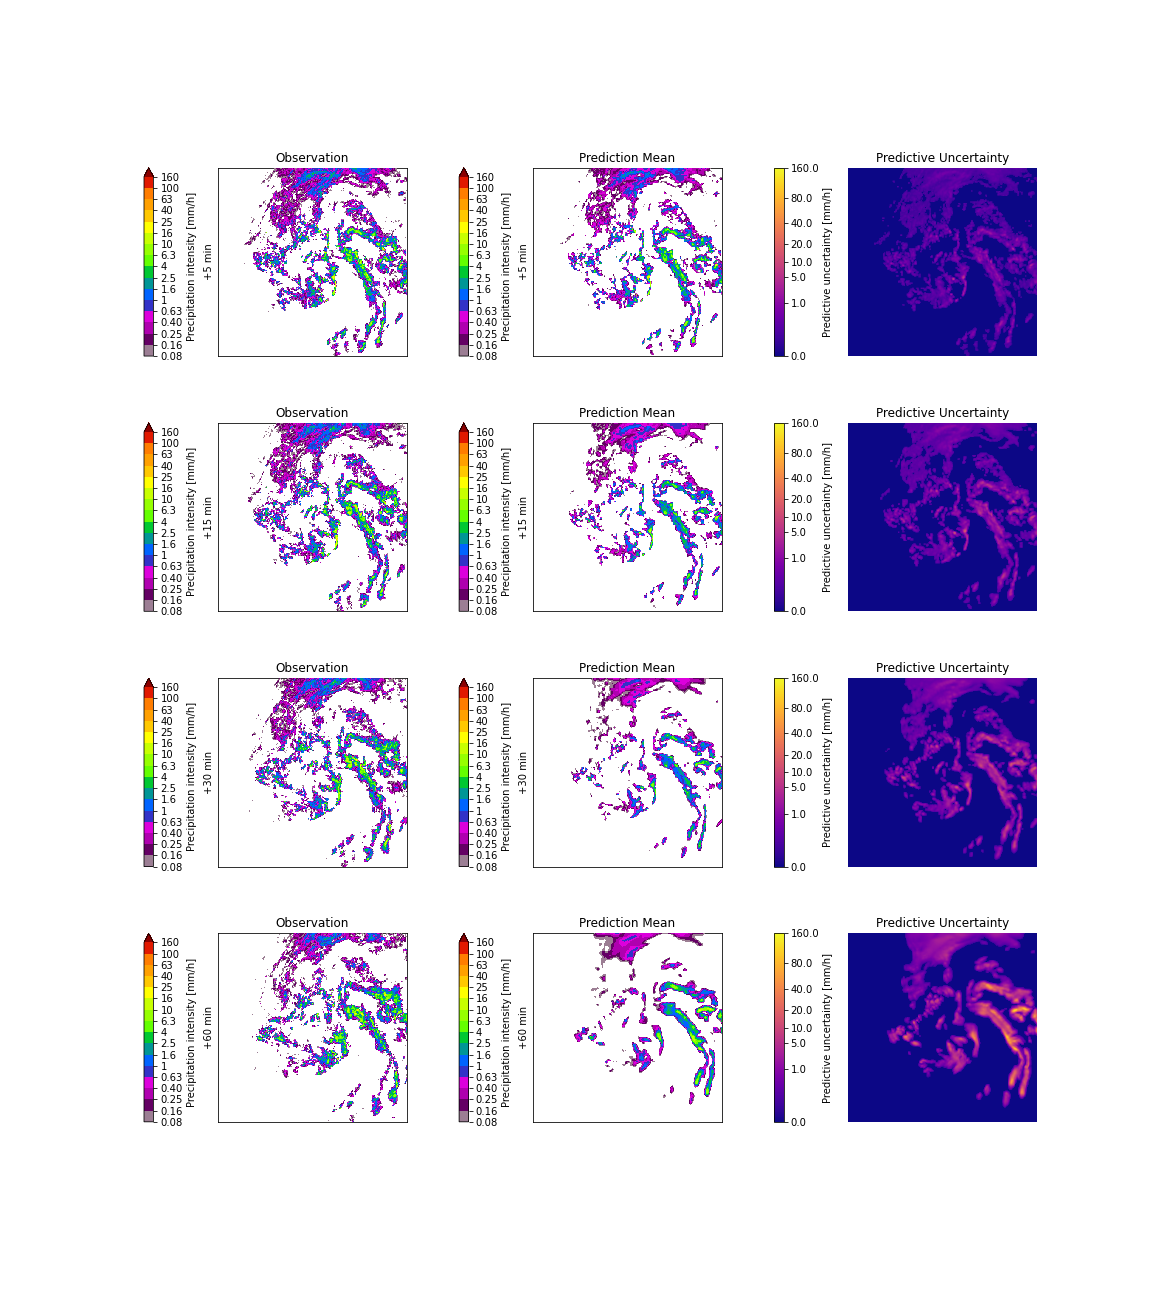
\includegraphics[width=1.4\textwidth]{images/cases/2019-05-25 13:00:00_bcnn_p2_lt5_lt5_15_30_60}
	\caption{case 1 2019-05-25 13:00:00}
\end{figure}

\subsection{Case study 2 : Rapidly evolving convective rain event}

%15.8.2021 afternoon
\begin{figure}
	\label{fig:case2_bcnn_lt5}
	\centering
	\hspace*{-1.5cm}
	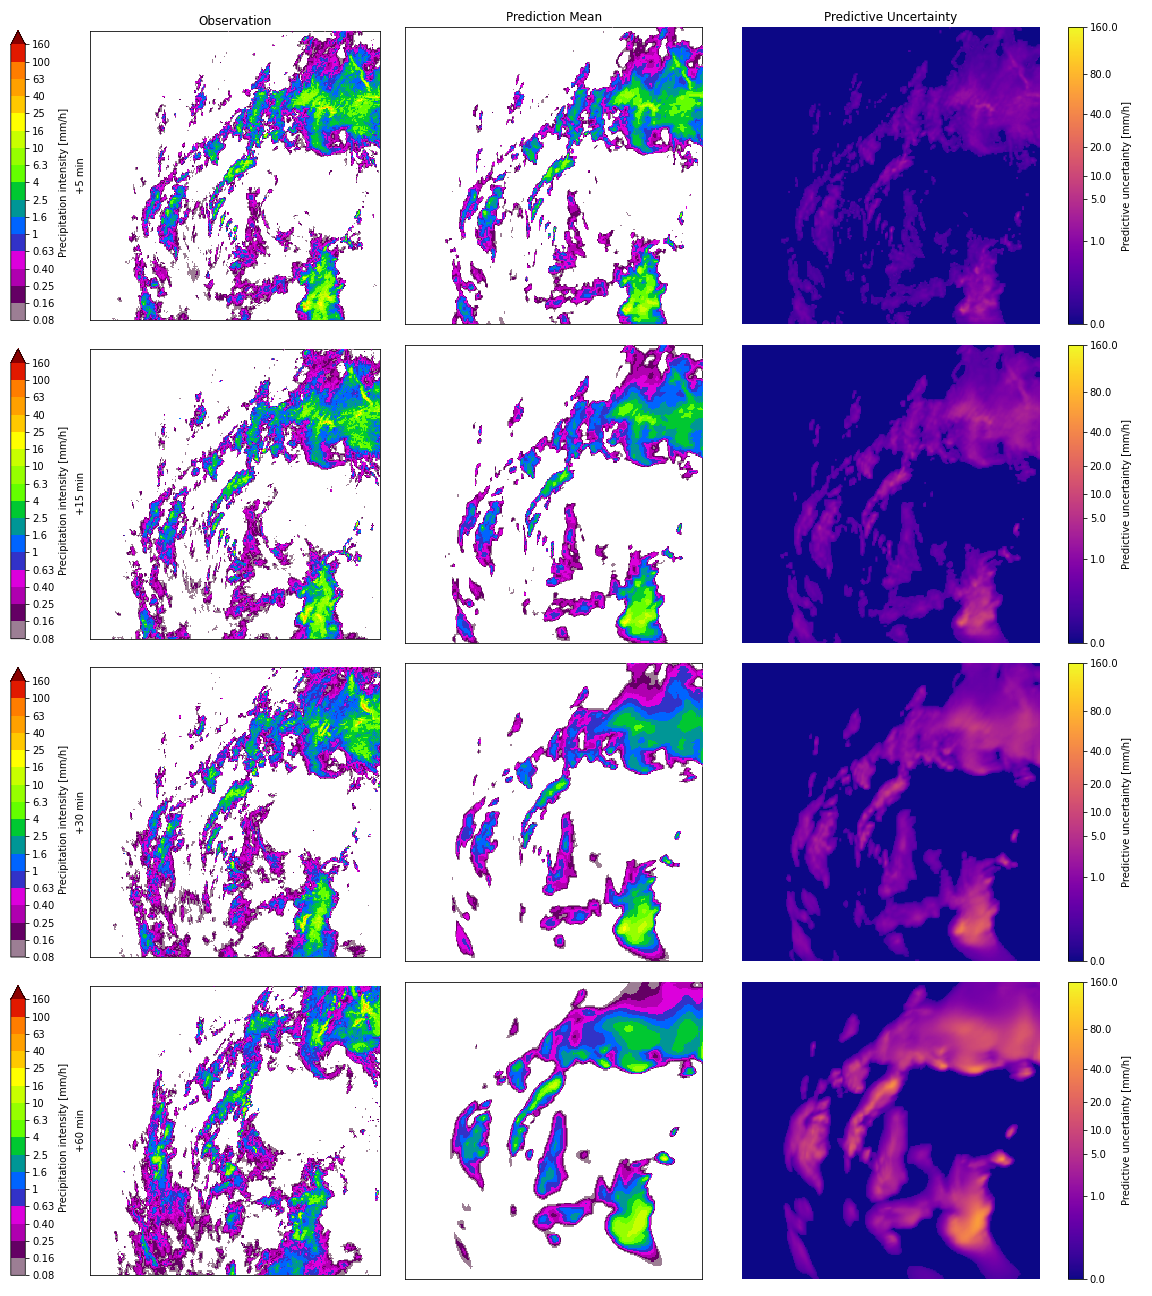
\includegraphics[width=1.2\textwidth]{images/cases/2021-05-18 21:00:00_bcnn_p2_lt5_lt5_15_30_60}
	\caption{case 2 2021-05-18 21:00:00}
\end{figure}


\section{Deterministic prediction skill (Metrics)}

\begin{figure}[ht]
	\label{fig:cont-metrics}
	\centering
	\subfloat[MAE]{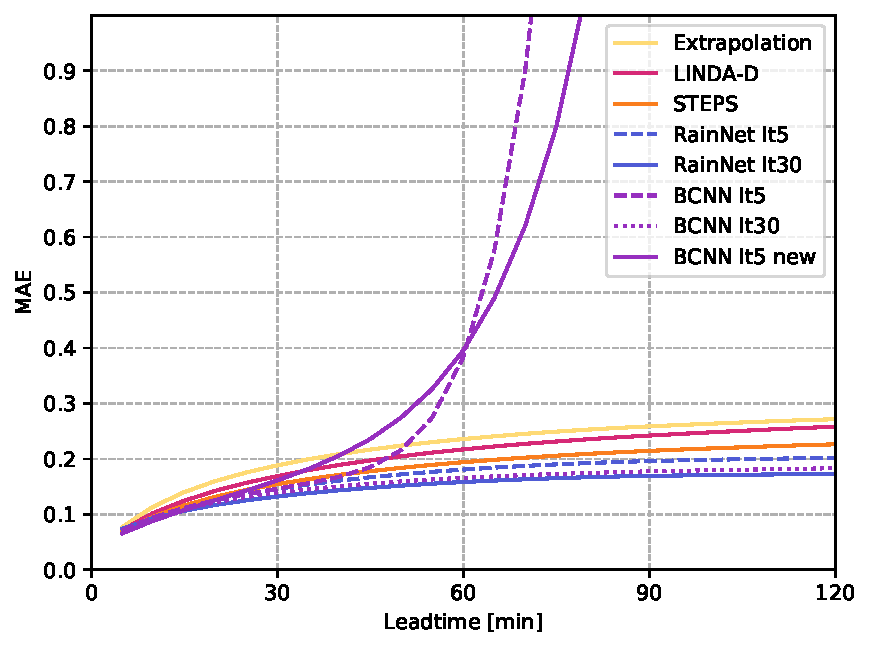
\includegraphics[width=0.5\textwidth]{images/metrics/ALL_MAE}}%
	\subfloat[ME]{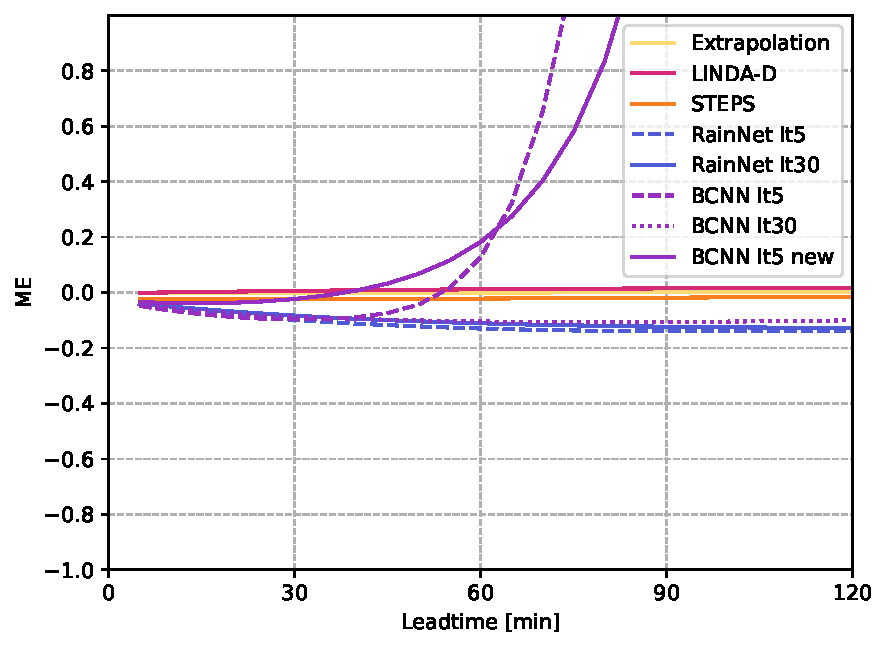
\includegraphics[width=0.5\textwidth]{images/metrics/ALL_ME}}%

	\caption{Continuous Metrics}
\end{figure}

\pagebreak

\begin{figure}
	\label{fig:cat-metrics}
	\centering
	\subfloat[ETS 0.5 mm/h]{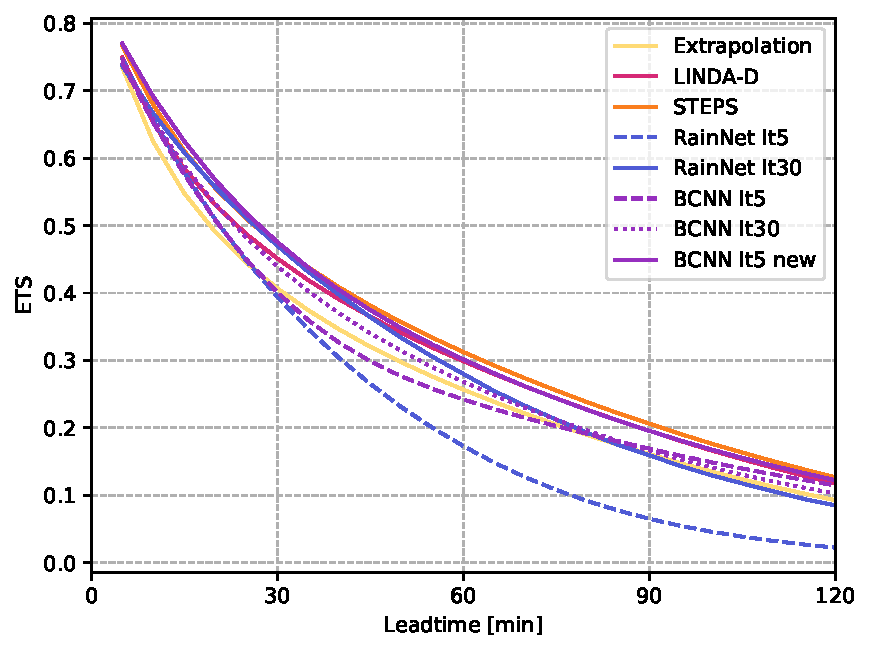
\includegraphics[width=0.35\textwidth]{images/metrics/ALL_ETS_0_5}}%
	\subfloat[ETS 5.0 mm/h]{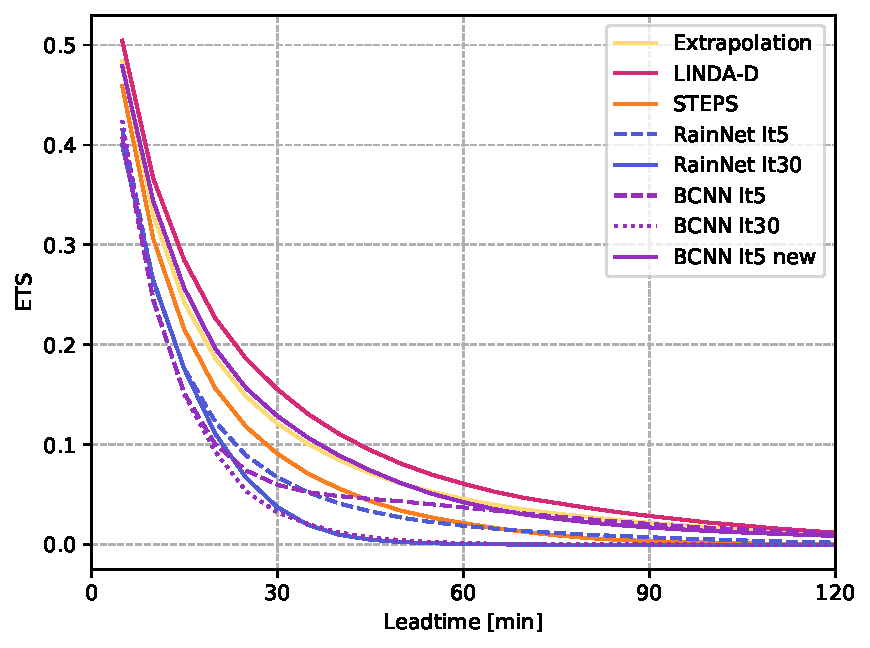
\includegraphics[width=0.35\textwidth]{images/metrics/ALL_ETS_5_0}}%
	\subfloat[ETS 20.0 mm/h]{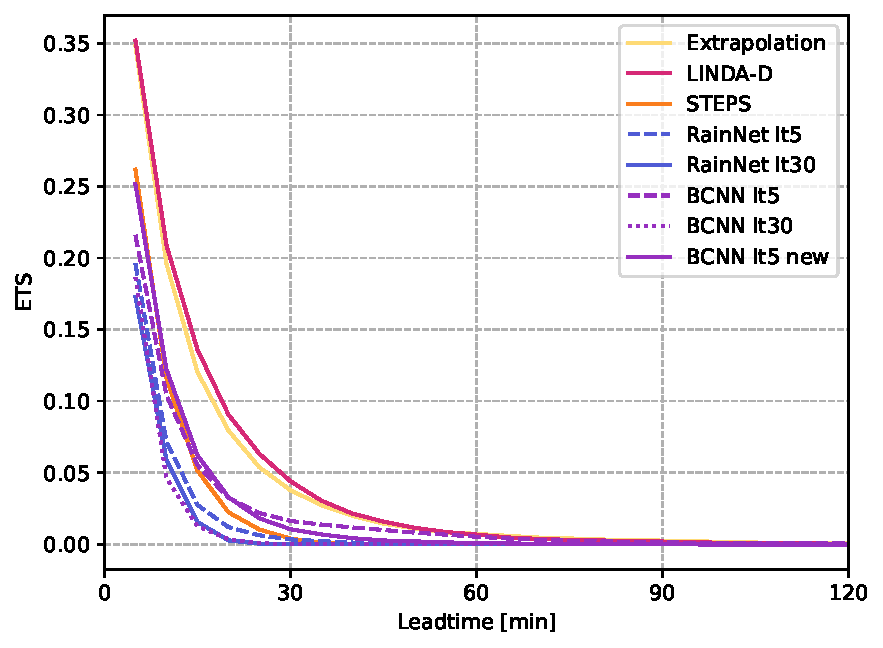
\includegraphics[width=0.35\textwidth]{images/metrics/ALL_ETS_20_0}}%
	
	
	
	\subfloat[FAR 0.5 mm/h]{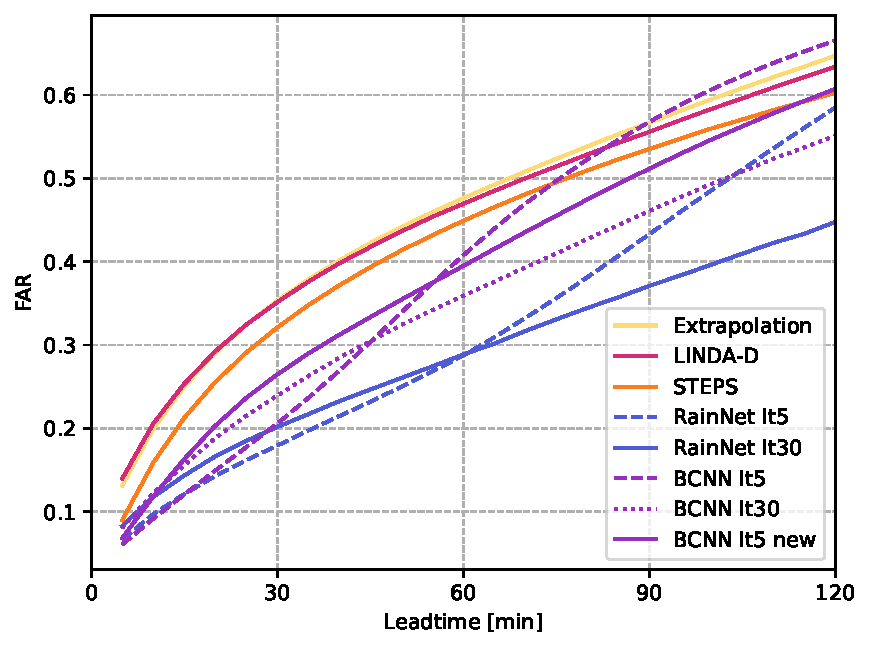
\includegraphics[width=0.35\textwidth]{images/metrics/ALL_FAR_0_5}}%
	\subfloat[FAR 5.0 mm/h]{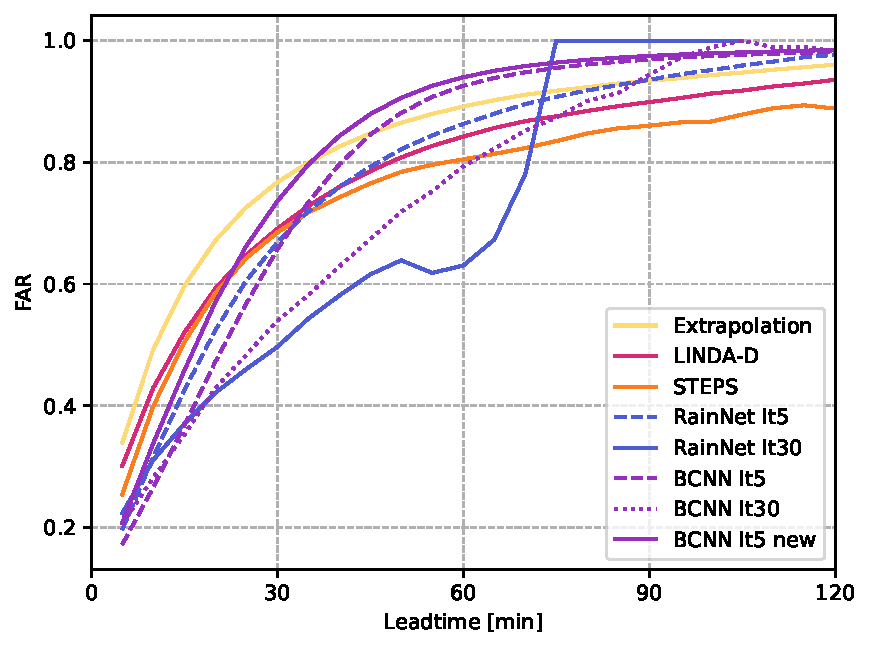
\includegraphics[width=0.35\textwidth]{images/metrics/ALL_FAR_5_0}}%
	\subfloat[FAR 20.0 mm/h]{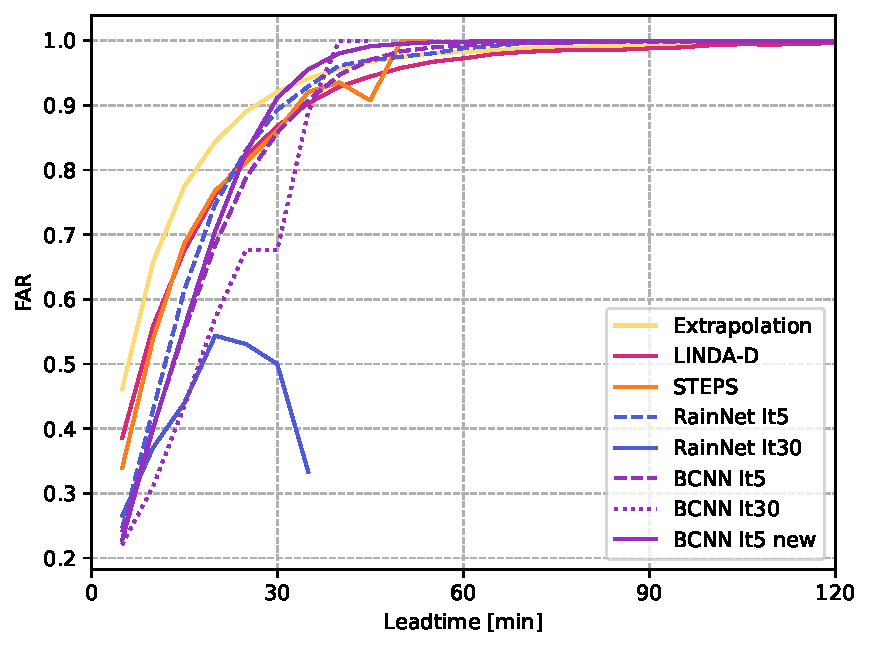
\includegraphics[width=0.35\textwidth]{images/metrics/ALL_FAR_20_0}}%
	
	\subfloat[POD 0.5 mm/h]{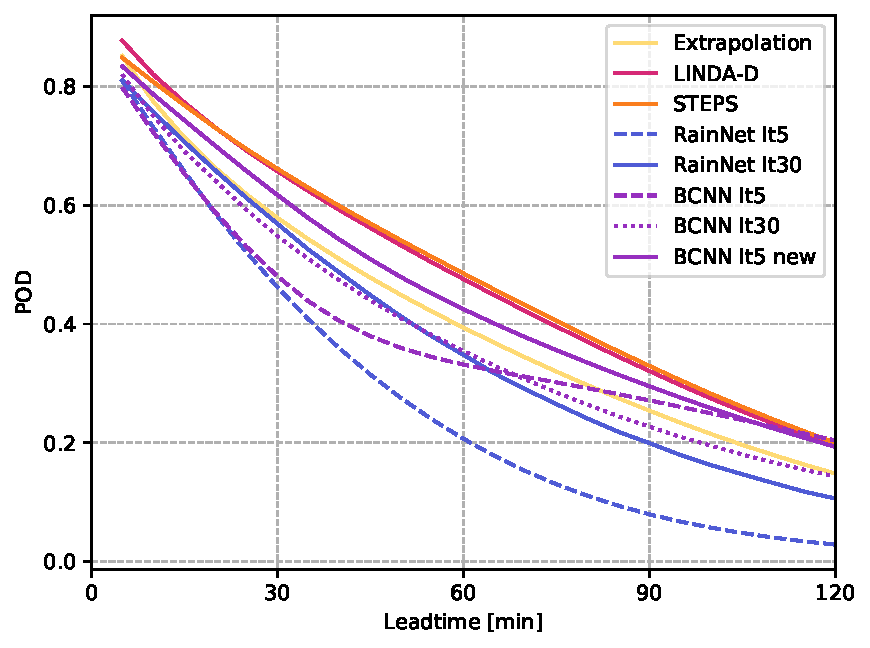
\includegraphics[width=0.35\textwidth]{images/metrics/ALL_POD_0_5}}%
	\subfloat[POD 5.0 mm/h]{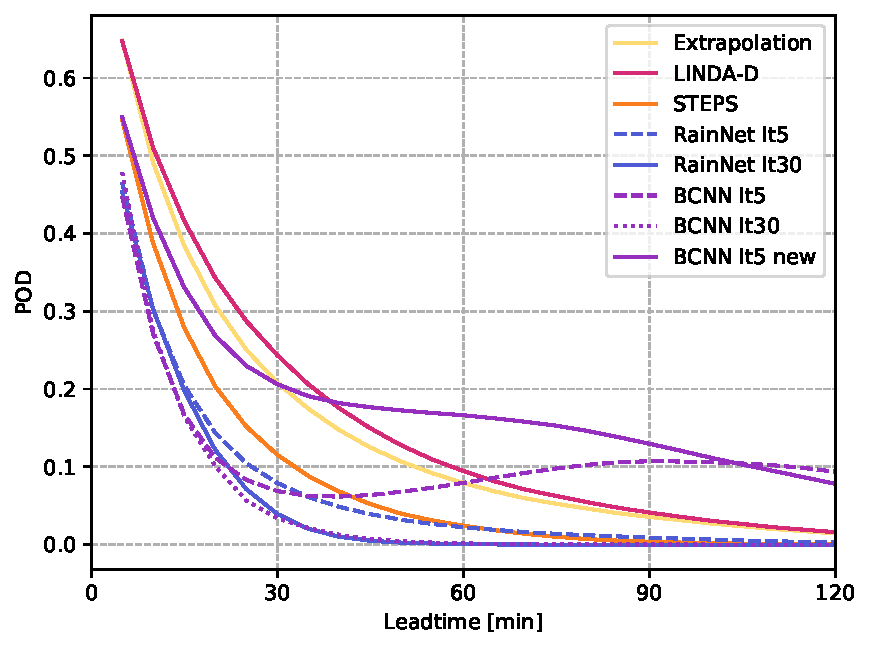
\includegraphics[width=0.35\textwidth]{images/metrics/ALL_POD_5_0}}%
	\subfloat[POD 20.0 mm/h]{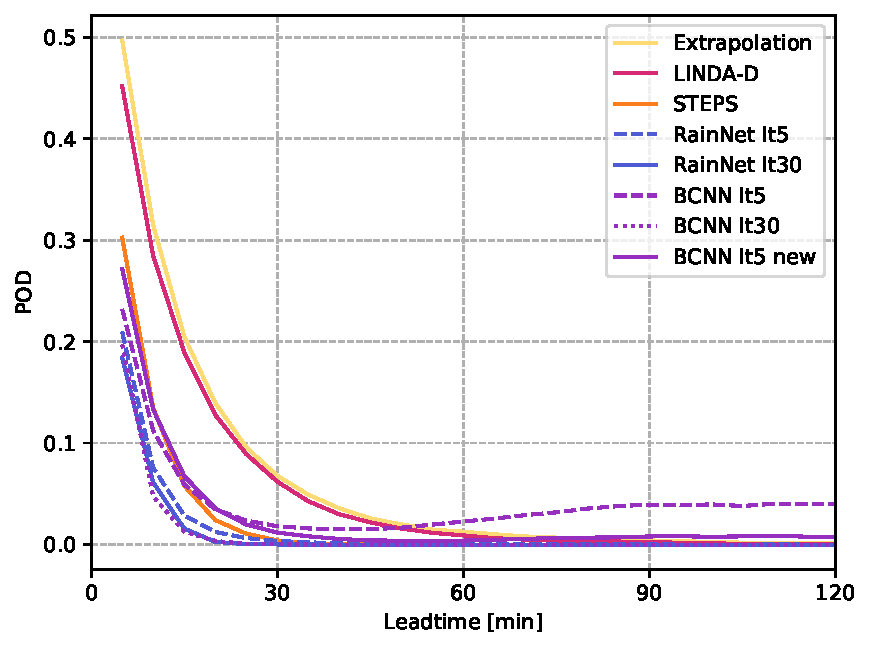
\includegraphics[width=0.35\textwidth]{images/metrics/ALL_POD_20_0}}%
	\caption{Categorical metrics}
	
\end{figure}


\begin{figure}[ht]
	\label{fig:fss16}
	\subfloat[0.5 mm/h]{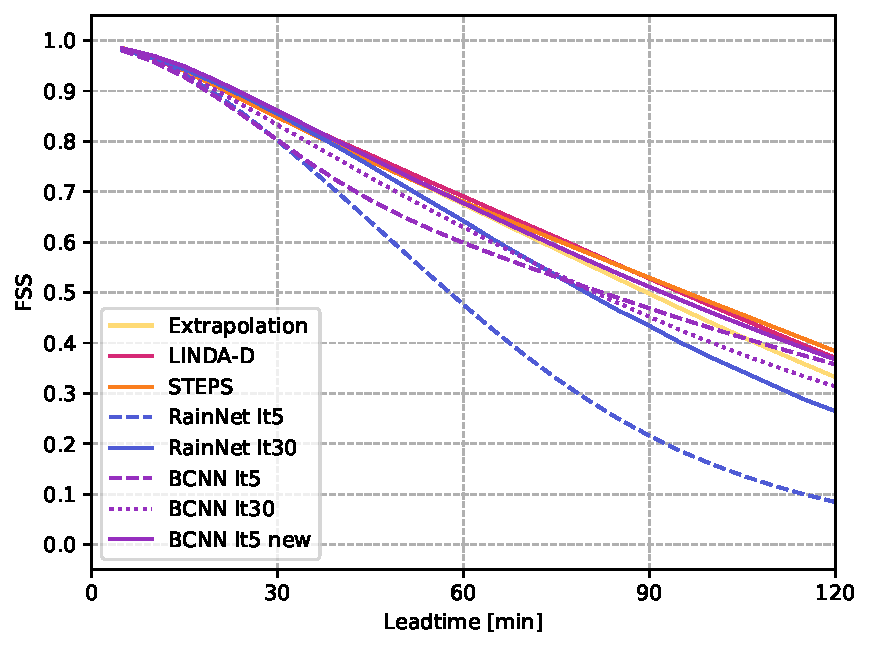
\includegraphics[width=0.33\textwidth]{images/metrics/ALL_FSS_8_0_5}}%
	\subfloat[5.0 mm/h]{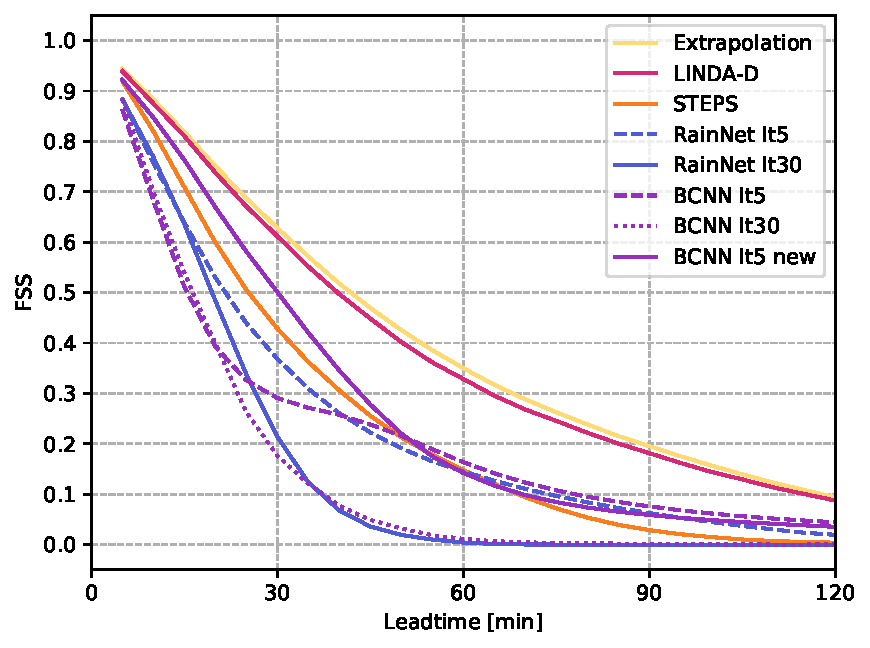
\includegraphics[width=0.33\textwidth]{images/metrics/ALL_FSS_8_5_0}}%
	\subfloat[20.0 mm/h]{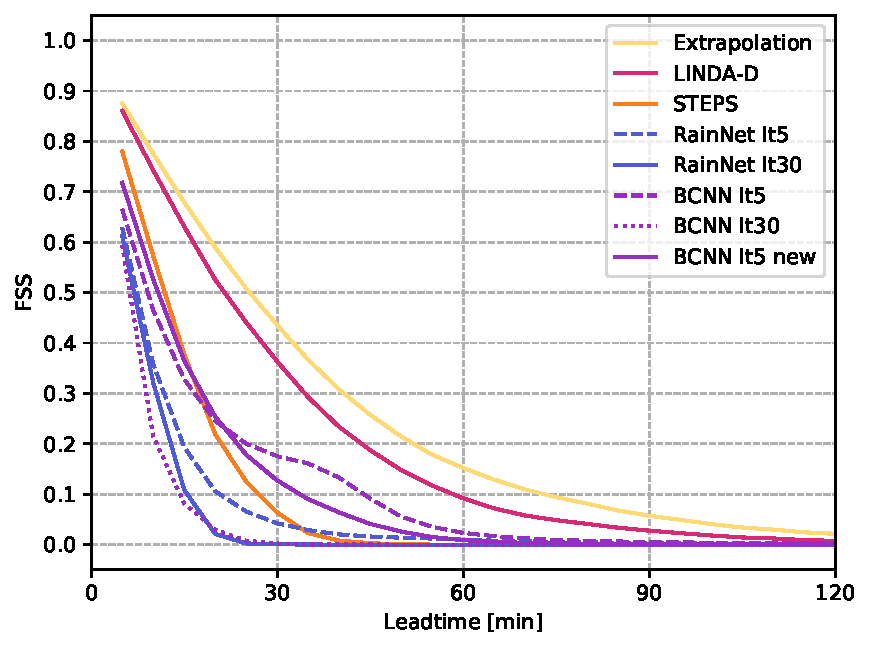
\includegraphics[width=0.33\textwidth]{images/metrics/ALL_FSS_8_20_0}}%
	\caption{FSS scores (16km)}
\end{figure}

\begin{figure}
	\label{fig:rapsd}
	\centering
	\subfloat[15 min]{
	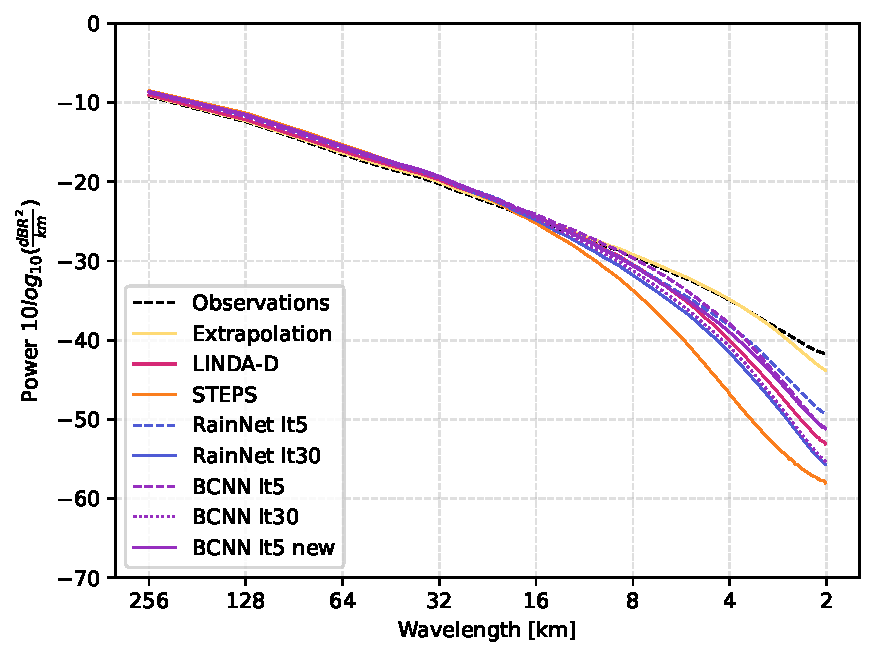
\includegraphics[width=0.33\textwidth]{images/metrics/ALL_15min_RAPSD}
}
	\subfloat[60 min]{
		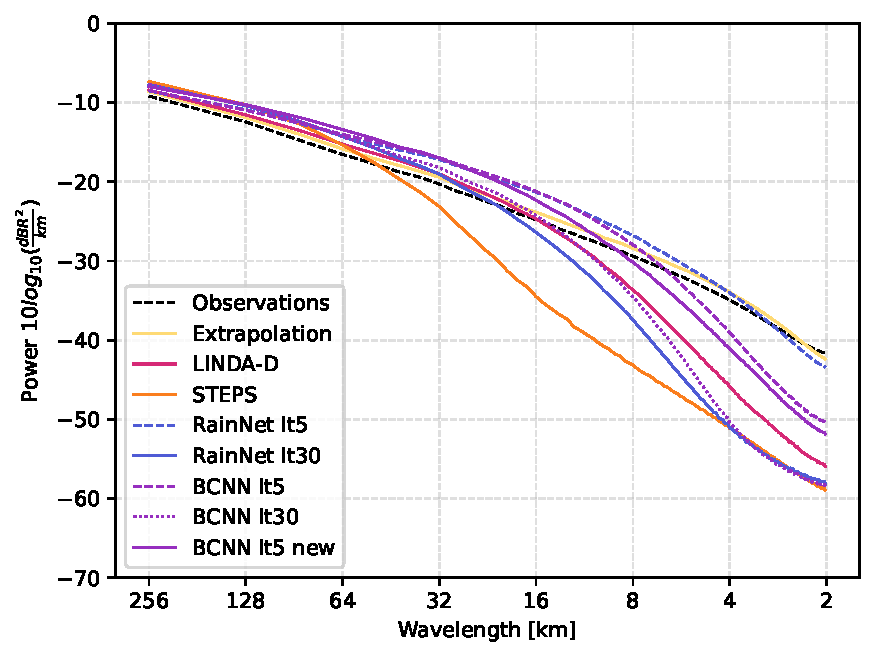
\includegraphics[width=0.33\textwidth]{images/metrics/ALL_60min_RAPSD}
	}
	\subfloat[120 min]{
		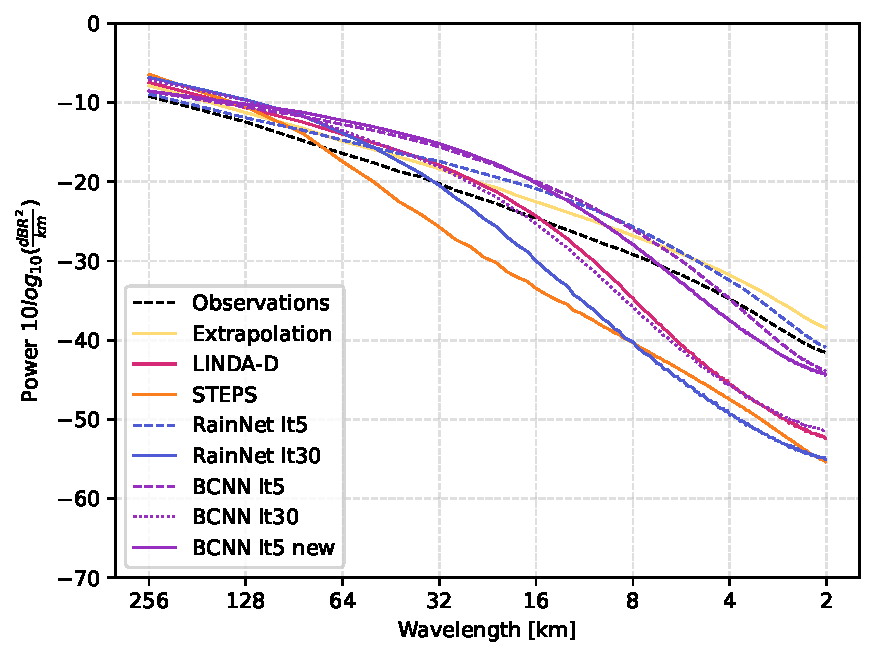
\includegraphics[width=0.33\textwidth]{images/metrics/ALL_120min_RAPSD}
	}
	\caption{RAPSD}
\end{figure}

\pagebreak
\section{Probabilistic prediction skill (Metrics)}

\begin{figure}
	\label{fig:crps}
	\centering
	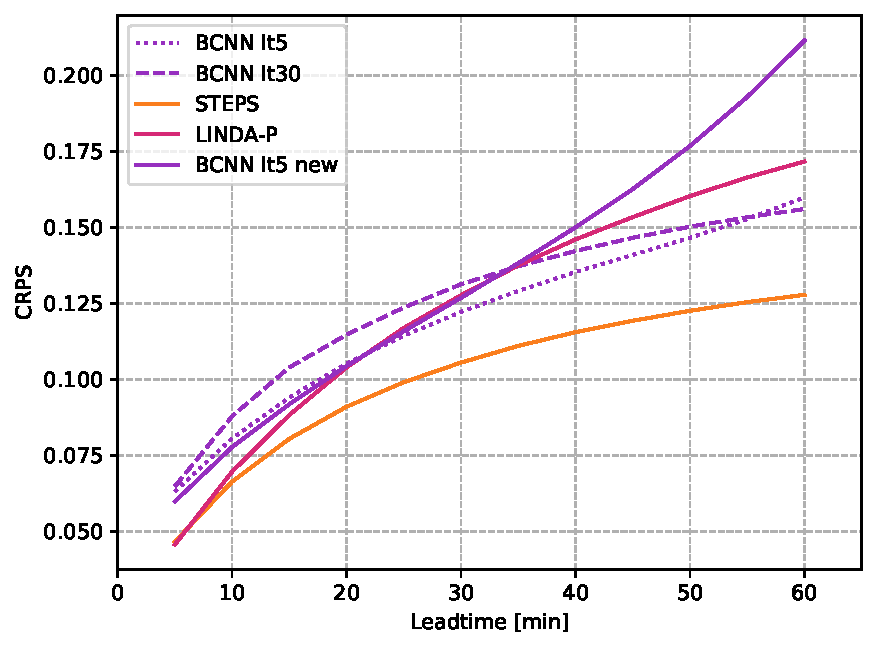
\includegraphics[width=0.6\linewidth]{images/metrics/ALL_CRPS}
	\caption{CRPS}
\end{figure}

text

\begin{figure}
	\label{fig:prob-metrics}
	\subfloat[ROC 0.5 mm/h]{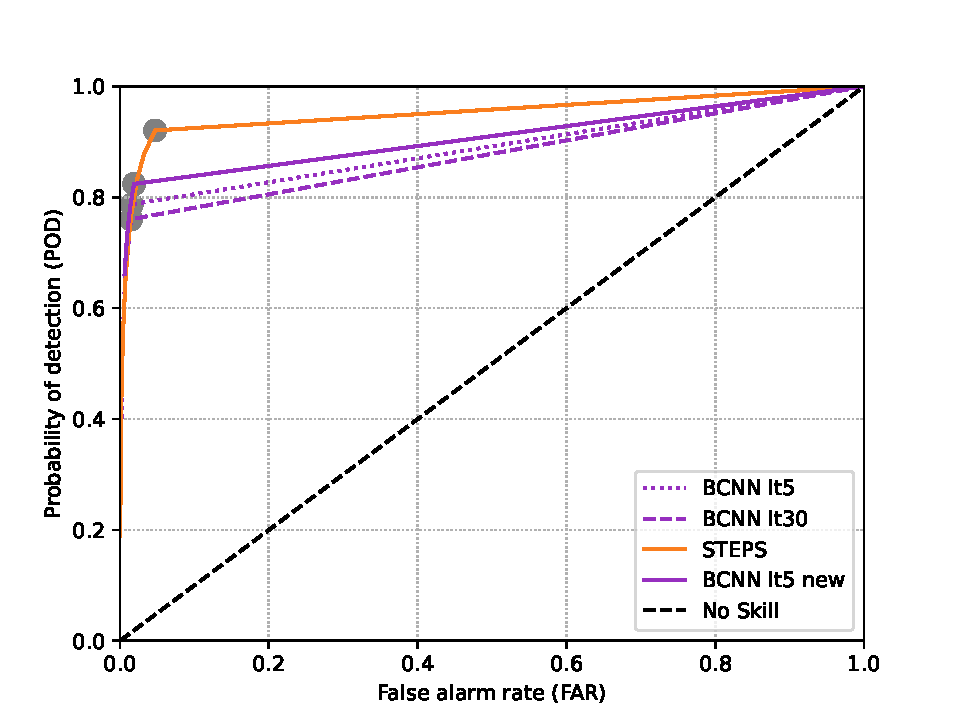
\includegraphics[width=0.33\textwidth]{images/metrics/ALL_ROC_l_12_t_0.5}}%
	\subfloat[ROC 5.0 mm/h]{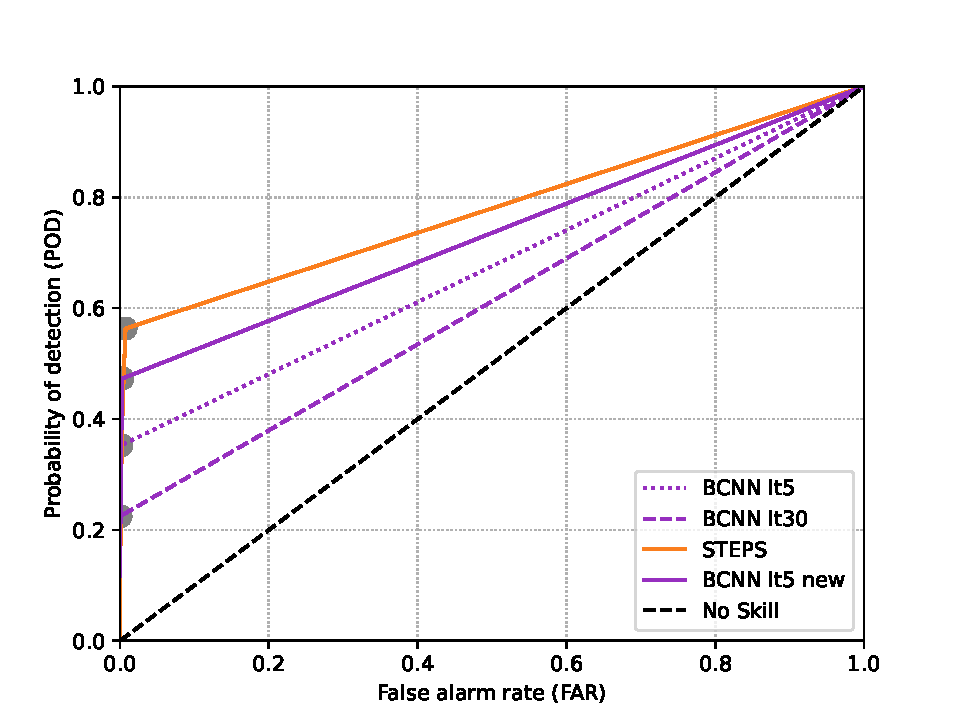
\includegraphics[width=0.33\textwidth]{images/metrics/ALL_ROC_l_12_t_5.0}}%
	\subfloat[ROC 20.0 mm/h]{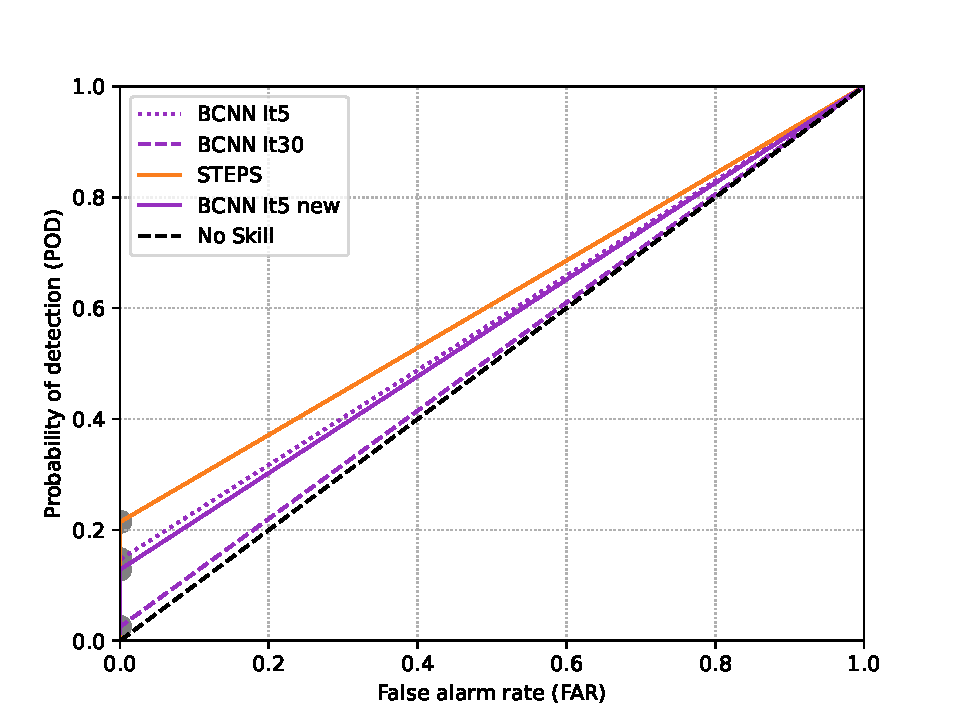
\includegraphics[width=0.33\textwidth]{images/metrics/ALL_ROC_l_12_t_20.0}}%
	
	
	
	\subfloat[RELDIAG 0.5 mm/h]{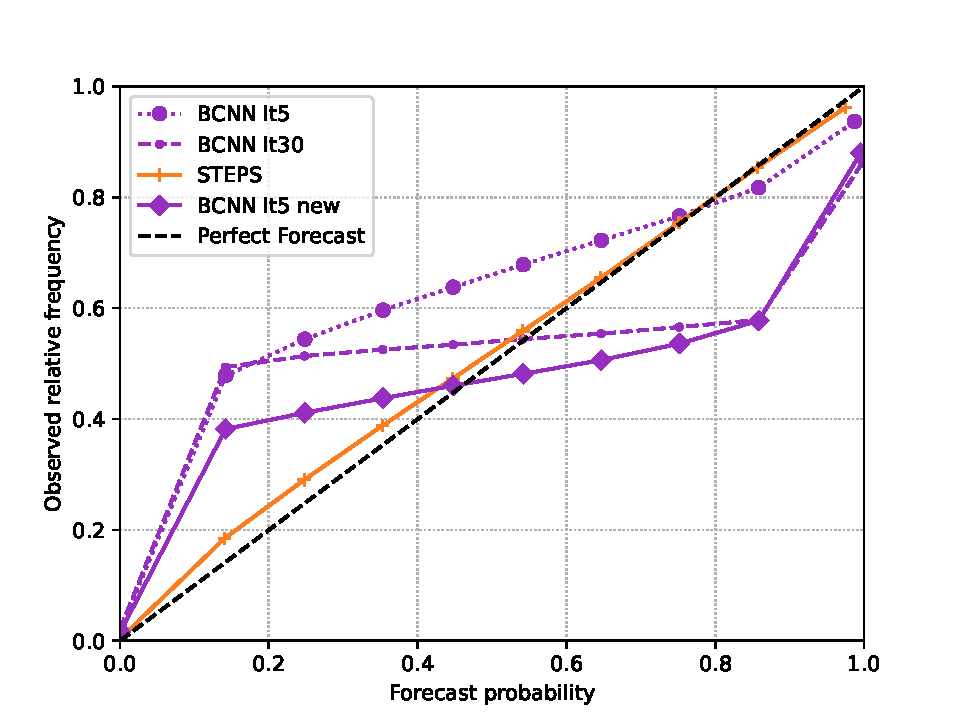
\includegraphics[width=0.33\textwidth]{images/metrics/ALL_RELDIAG_l_12_t_0.5}}%
	\subfloat[RELDIAG 5.0 mm/h]{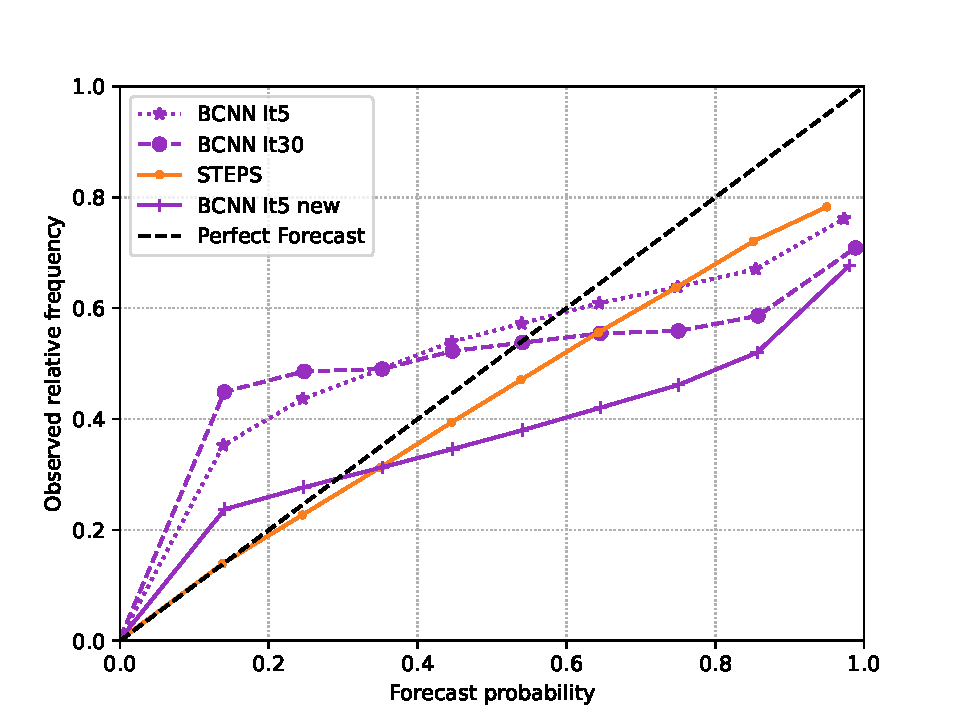
\includegraphics[width=0.33\textwidth]{images/metrics/ALL_RELDIAG_l_12_t_5.0}}%
	\subfloat[RELDIAG 20.0 mm/h]{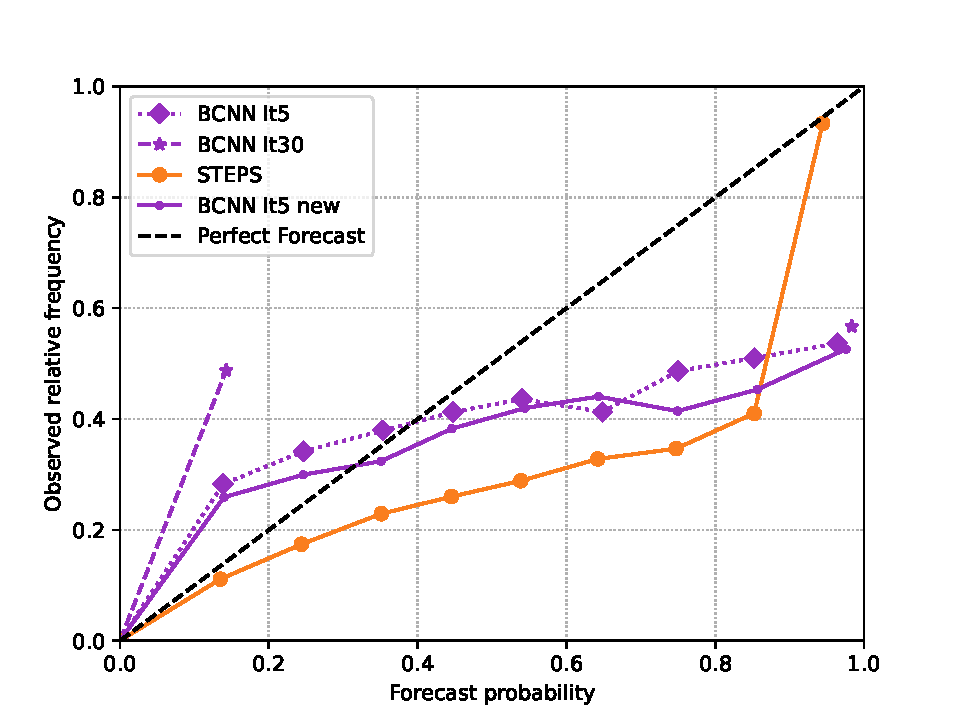
\includegraphics[width=0.33\textwidth]{images/metrics/ALL_RELDIAG_l_12_t_20.0}}%
	\caption{ROC curves and Reliability diagrams for a one-hour forecast at different precipitation thresholds.}
\end{figure}


\begin{figure}
	\label{fig:rh}
	\centering
	\subfloat[BCNN lt5]{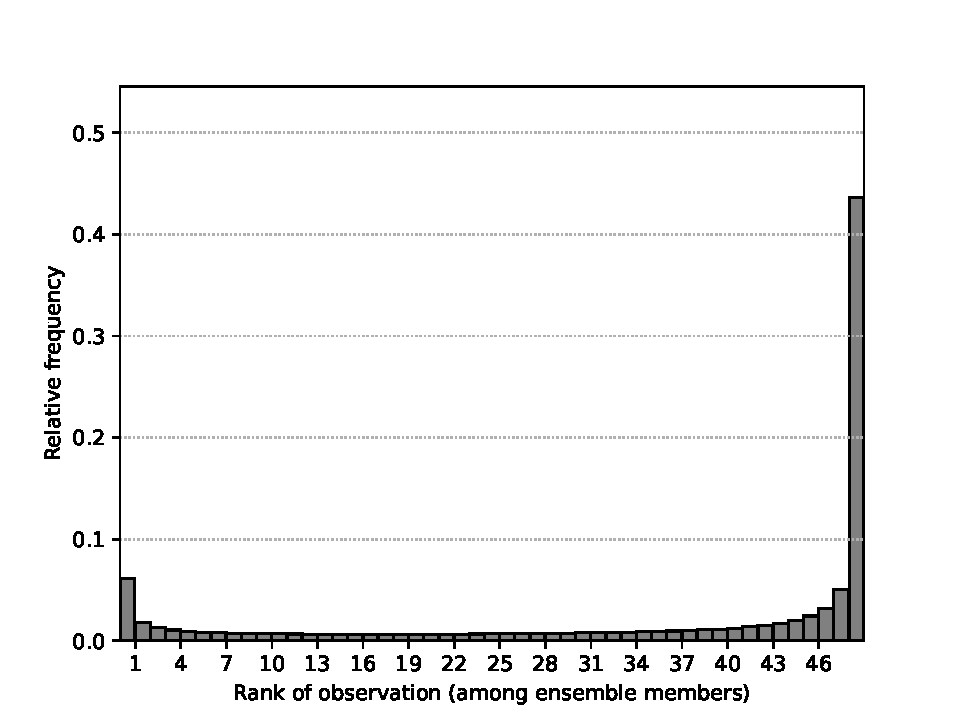
\includegraphics[width=0.5\textwidth]{images/metrics/bcnn_p2_lt5_rankhist_l_12}}%
	\subfloat[BCNN lt30]{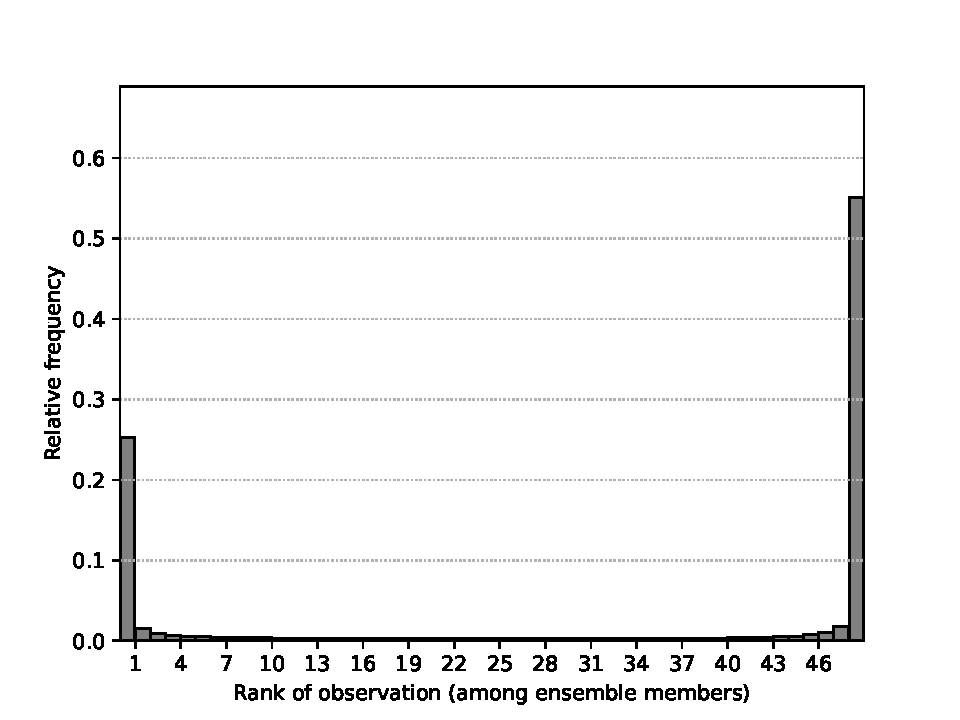
\includegraphics[width=0.5\textwidth]{images/metrics/bcnn_p2_lt30_rankhist_l_12}}%
	
	\subfloat[BCNN lt5 new]{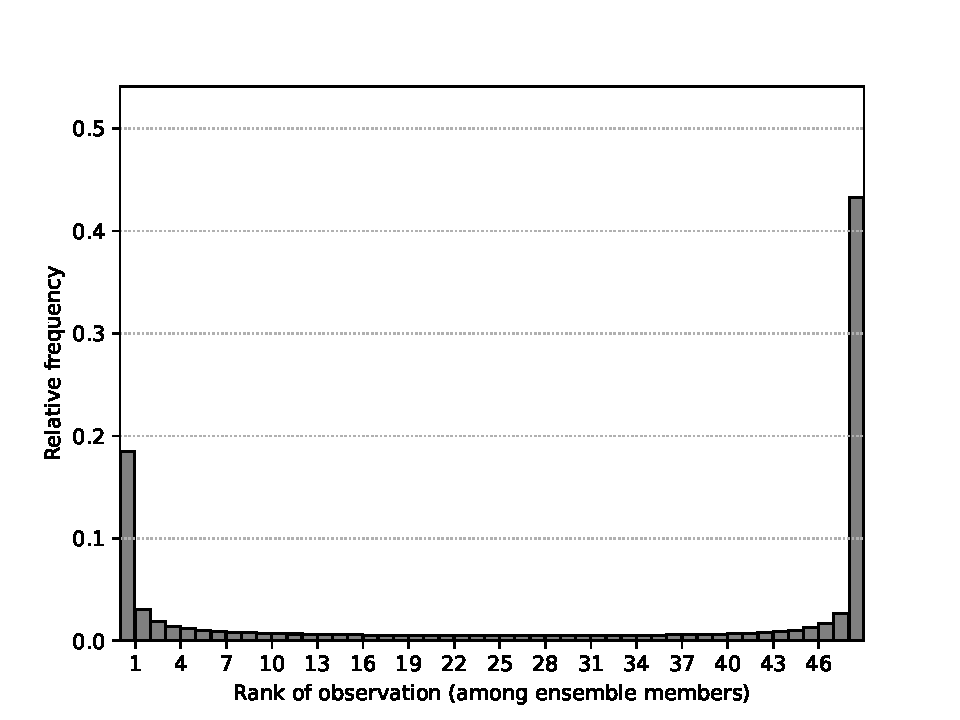
\includegraphics[width=0.5\textwidth]{images/metrics/bcnn_sdb_bs2_lt5_last_rankhist_l_12}}%
	\subfloat[STEPS]{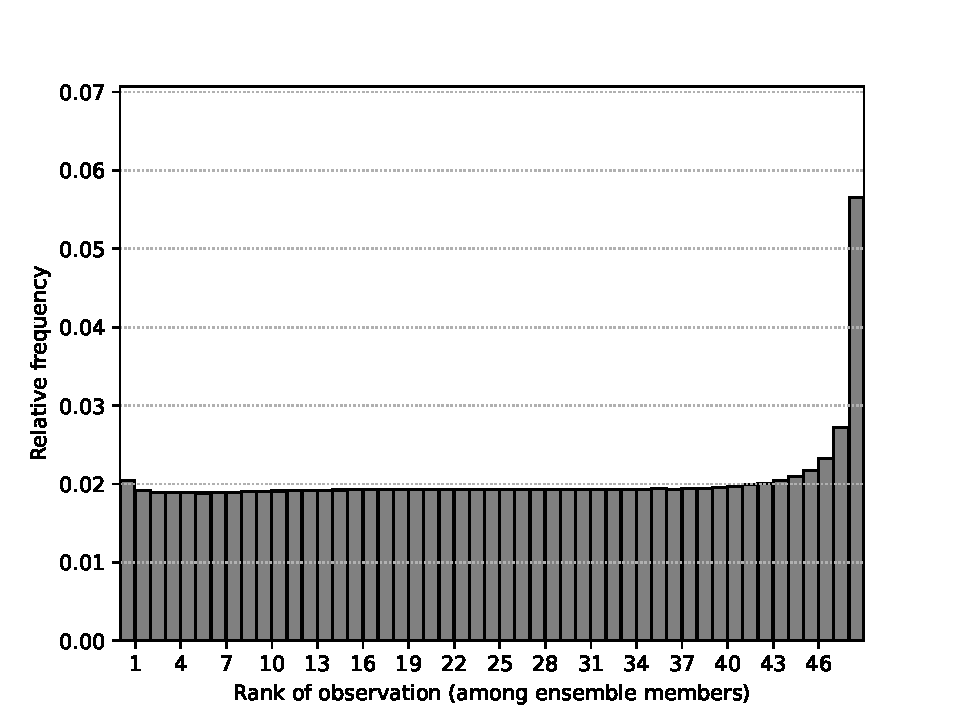
\includegraphics[width=0.5\textwidth]{images/metrics/steps_rankhist_l_12}}%
	
	\caption{Rank histograms for probabilistic models.}
\end{figure}

\begin{figure}
	\label{fig:rh}
	\centering
	\subfloat[BCNN lt5]{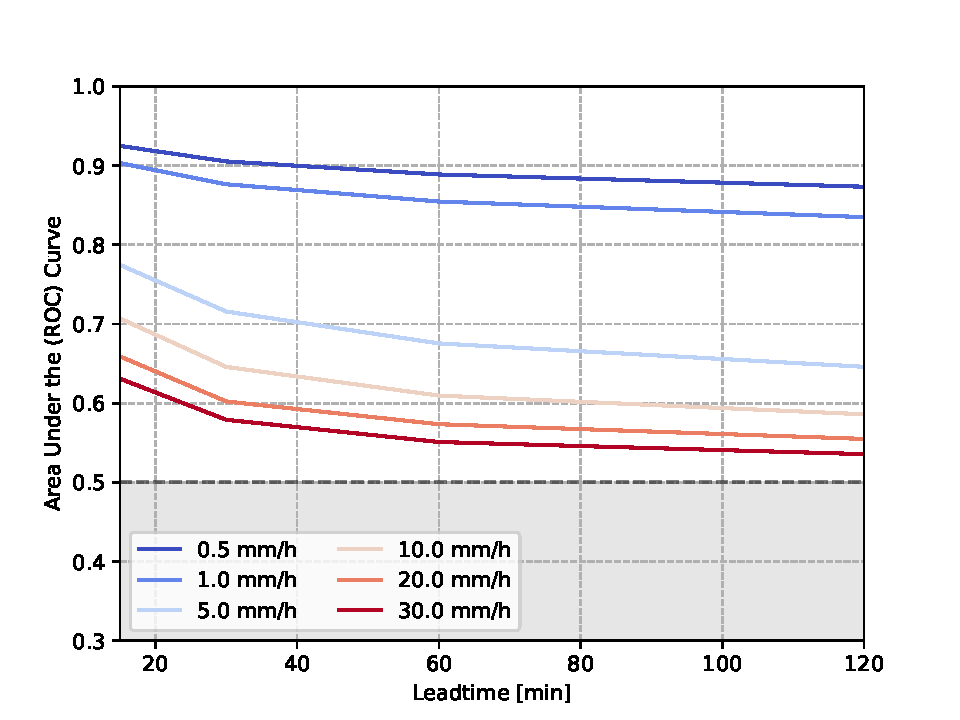
\includegraphics[width=0.5\textwidth]{images/metrics/bcnn_p2_lt5_AUC}}%
	\subfloat[BCNN lt30]{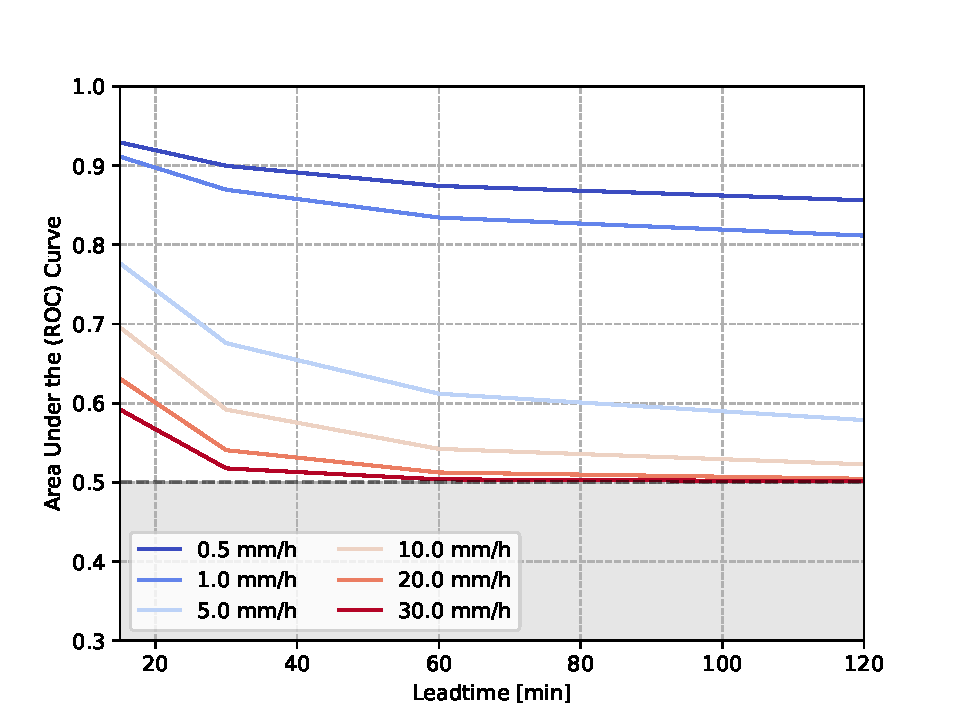
\includegraphics[width=0.5\textwidth]{images/metrics/bcnn_p2_lt30_AUC}}%
	
	\subfloat[BCNN lt5 new]{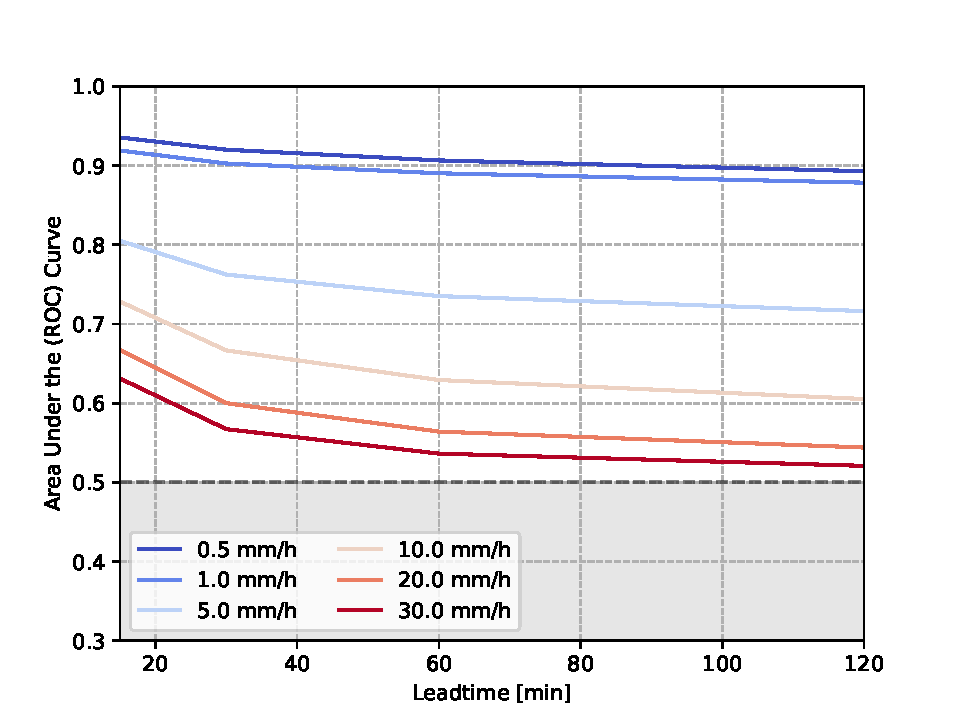
\includegraphics[width=0.5\textwidth]{images/metrics/bcnn_sdb_bs2_lt5_last_AUC}}%
	\subfloat[STEPS]{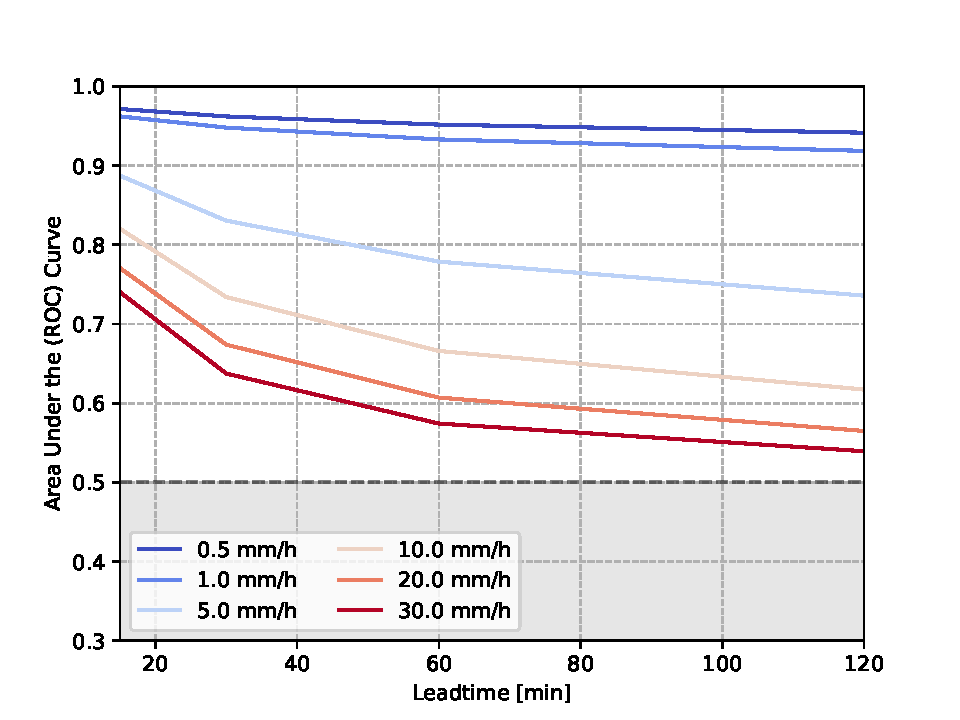
\includegraphics[width=0.5\textwidth]{images/metrics/steps_AUC}}%
	
	\caption{ROC Area under the curves summarized for probabilistic models.}
\end{figure}

 
